We will now provide an overview of the two main concepts that, when combined,
drive the motivation behind the inception and development of this project.

\subsection{Data mining}
\label{Introduction::Context::DataMining}

Information society produces vast amounts of data all over the world.
This data comes from innumerable sources and in diverse formats, and has been stored 
for years in data warehouses, waiting to be processed. With the continuous increase 
in computing power, due to the recent advances in software and hardware technologies, 
the machine learning field, more commonly known as \textit{data mining}, has arisen, 
allowing us to exploit this stored data and distill knowledge from it.

Data mining is, indeed, a holistic process, where many different disciplines are 
involved, from data acquisition and storage, through its selection, filtering and 
analysis up to information extraction, visualization and knowledge discovery.

\begin{figure}[h]
	\centering
	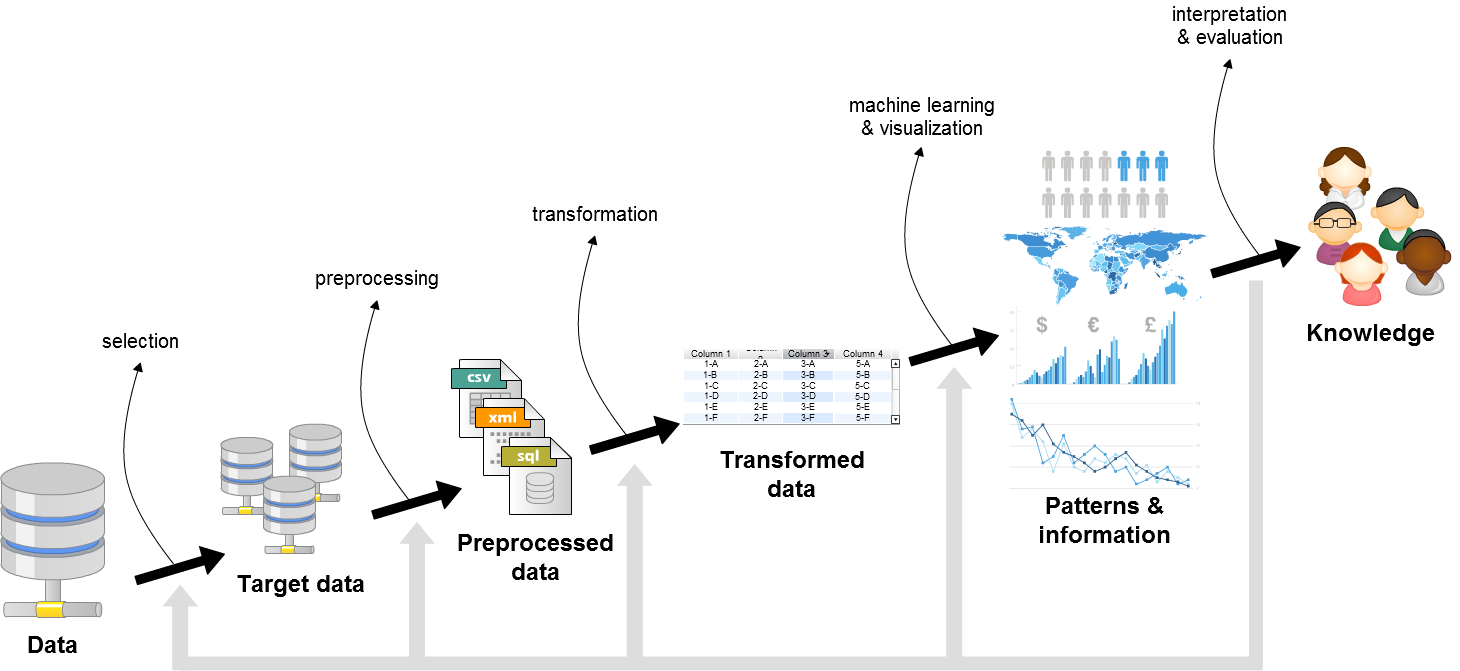
\includegraphics[width=0.9\linewidth]{Figures/data-mining-process.png}
	\caption{Data mining as a process. Adapted from~\citet{Fayyad:FromDataMining}}
	\label{fig:data-mining}
\end{figure}

Data mining enables a better understanding of human or natural processes and provides 
us with means to identify trends, predict future events or discover useful patterns. 
Its uses range from scientific and medical applications to social sciences or business
administration~\citep{Fayyad:FromDataMining}.

\subsubsection{Facing the limits}

Despite lots of effort is put into enhancing different data mining processes, there still 
are many cases where these techniques fail to perform correctly; mainly, it is a matter of scale.

On one hand, traditional data mining workflows cannot cope with the really massive 
data sets that are available nowadays, if performed on a common infrastructure. 
To solve this issue, clusters of hundreds or thousands of computers are used to run 
such analysis. It is costly and complex but, doing so, we can mine data that we could not 
some time ago.

On the other hand, we face another type of scaling problem. In some situations, data 
acquisition throughput is so high that it cannot be stored anyway, so another approach 
is needed to avoid the loss of information that it could deliver us. Moreover, we might 
not want to store it, even when we could, but yet we want to analyze it to extract 
knowledge from it, as soon as we received it. Both these scenarios are addressed with a 
series of techniques known as \textit{stream mining}.

\subsubsection{Stream mining}

\textit{Stream mining} or \textit{data stream mining} is a process that allows us to 
still discover knowledge and patterns in data, even when it comes in the form of a 
continuous stream, or many of them~\citep{Rajaraman:MiningMassiveDatasets}. Instead of processing 
all statically stored data, like traditional data mining does, a relatively small 
portion of it is kept during the analysis, and it is updated when needed - either because 
more resources are available to the system or because new data is acquired. A more deeper 
review of this research area is given in \sref{NULL}.

\subsection{Privacy}
\label{Introduction::Context::Privacy}

Privacy is a concept that can be defined as the ability of an individual or group to 
seclude\footnote{“Seclusion is the act of placing or keeping someone away from other people.”~\citep{web:Merriam:Seclusion}} themselves, or information about themselves, and 
thereby express themselves selectively. It is understood differently depending on the social 
and cultural background of each individual, but it is in fact recognised as one of the most 
fundamental rights of our human nature. The Universal Declaration of Human Rights’ 12th 
article~\citep{web:UN:HumanRightsDeclaration} states that:

\begin{quote}
	No one shall be subjected to arbitrary interference with his privacy, family, home or 
	correspondence, nor to attacks upon his honour and reputation. Everyone has the right to 
	the protection of the law against such interference or attacks.
\end{quote}

This right has been continuously violated ever since information exchange and advanced 
communication technologies have been developed. Despite this did not begin with the spread 
of the Internet, its adoption has greatly magnified both the ability to breach people’s privacy 
and the impact that these breaches have. A more thorough analysis of privacy and its interrelations
with society and technology is given in \sref{NULL}.

\subsection{Privacy Preserving Data Mining}
\label{Introduction::Context::PPSM}

Data mining technologies have become a relevant debate topic nowadays, concerning what 
information is collected from individuals, who owns it and what are the purposes behind 
its gathering. Information technologies deliver us many benefits at many levels - safer 
streets, cheaper communications, better health systems, more convenient shopping - but 
at the high cost of losing our privacy.

Knowledge discovery processes need data to work and, in most cases, it is sensitive and 
personal. Moreover, it is massively collected and stored and analyzed without us knowing 
much about it. Besides the lack of consent in this data acquisition stage of the process, 
data mining poses a bigger thread on individuals: information disclosure. Sensitive data 
must be treated accordingly, which involves not only good IT security practices to avoid 
information leaks, but a responsible treatment when research results are published.

\subsubsection{Statistical Disclosure Control}

\textit{Statistical Disclosure Control} (SDC) is the name that the statistical community 
has given to what the data mining community calls Privacy Preserving Data Mining (PPDM). 
This field, whatever its preferred name is, deals with controlling that information about 
specific individuals is not extracted from statistical summary results. Also, if full 
datasets are to be released, PPDM methods should be applied to data in order to preserve 
user's privacy, whilst maintaining the statistical significance of it, i. e., the amount 
of information - knowledge - that this data can provide.